\documentclass{article}
\usepackage[margin=0.5in]{geometry}
\usepackage{graphicx}
\usepackage{subcaption}

\title{Rutgers CS 440 Homework 1}
\author{Fulton Wilcox III, Dan Teytel, Long Tran}
\date{February 17 2023}

\begin{document}

\maketitle

    \begin{enumerate}
        \item[1.] \textbf{Understanding the Methods}
        \begin{enumerate}

            \begin{figure}[h!]
			\IfFileExists{diagram.png}{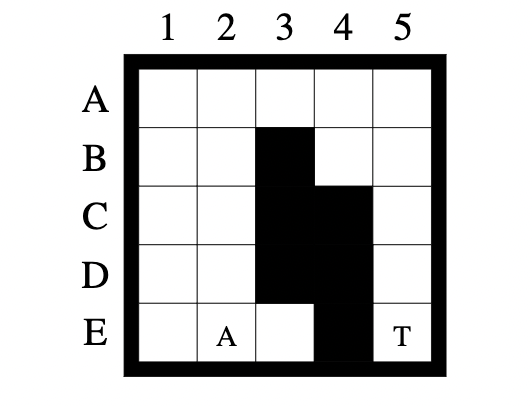
\includegraphics[width=0.2\textwidth]{diagram.png}}{No Figure Yet}
		\end{figure}
            
            \item[a.] In this example, the first move from A to the target will be to the right rather than up because the heuristic, which is the Manhattan distance from the current spot to the target, is 2 for the spot E3, while the heuristic for spot D2 is 4.  The step cost is 1 for both since this is the first step, so F(E3) $<$ F(D2).

            \item[b.] Using A* search, the agent either reaches the target or discovers that it is impossible to reach the target.
            To argue this, consider an agent and a target at any arbitrary spots on an arbitrarily generated maze.  An agent can expand its current node in any direction if that particular cell is unblocked and then move to the cell that has the lowest f(n).  Assuming the target is unreachable, as long as there is an unblocked cell adjacent to an expanded cell, A* will not terminate.  Therefore, in the worst case, A* will terminate only when there are no longer any adjacent un-expanded cells.  In the case when there is a path to the target, A* will terminate when every other path has greater cost than the cost to the target.  Let A represent an agent performing A* in a maze, M the total number of moves made by A, E be the number of expanded cells, and U the number of unblocked cells in the maze.
            \\
            \begin{enumerate}
            \item[Part 1] When A is using forward A*, each unblocked cell is only expanded once, and each move can only be made to a cell that has been expanded, meaning M $\le$ E $\le$ U $\le$ $U^2$, meaning M $\le$ $U^2$, proving M=O($U^2$) when A is performing forward A*.
            \\
            \item[Part 2] When A is using Adaptive A* or Repeated forward A*, A uses forward A* to generate a path through an unexplored maze, following that path until A reaches the goal or the path is blocked by a blocked cell. Let M(i) be the number of moves M in the "i"th iteration of A*. Since A stops when a blocked cell is in the path and does not enter any blocked cell or repeatedly enter an unblocked cell in the same iteration of A*, the statement M(i)$\le$ U still holds for the path proposed by A* for the unknown maze despite E $\le$ U not necessarily being true. Additionally, since A remembers the status of each cell adjacent to a visited cell and uses that status to generate a path with A*, and A* only stops on its path if the next cell in the path is blocked or the target, A will never stop at a given cell twice since A* would never create a path through a known blocked cell. 
            \end{enumerate}
        \end{enumerate}
        \item[2.] \textbf{The Effects of Ties}
            \begin{enumerate}
                \item[] In the experiment, we conducted 50 random mazes and counted the average number of nodes expanded by Repeated A* using both tie breakers. The results have a very large difference as the tie breaker favoring smaller g(x) expands 100 times more nodes than its opposite. [Figure.\ref{TieBreakerNumber}]
                
                \begin{figure}[h!]
                    \centering
                    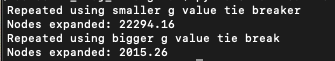
\includegraphics[width=.4\linewidth]{tie-breaker-number.png}
                    \caption{Comparison of Number of Nodes Expanded}
                    \label{TieBreakerNumber}
                \end{figure}
                
                \item[] There is a significant difference in the tie breakers between favoring cells with larger g-values and favoring cells with smaller g-values. 
                Tie-breaking favoring cells with the smaller g-values expands significantly more nodes. Using this tie breaker, the algorithm seems to explore more unnecessary cells and is less focused towards the target. On the other hand, the tie breaker favoring the larger g-values gives a far more focused path toward the target, and runs much faster as a result. [Figure.\ref{tie-breaker}]
                

                \item[] \textbf{Reason of the difference:}
                Since the evaluation function is $f(x) = g(x) + h(x)$, where g(x) is the step cost, favoring the smaller g-value whenever the evaluation values are equals ($f(x_1) = f(x_2)$) will lead the algorithm to explore cells that are closer to the start position. Therefore, the exploration pattern looks like the pattern of Breadth-First Search, since the algorithm prioritizes the cells closer to the start position.
                \item[] Otherwise, favoring larger g-values will explore the cells that are farthest from the start position. Combining this with the heuristic will result in the algorithm exploring cells farther from the start and towards the target.
                \item[] In conclusion, it is obvious that using the tie breaker favoring larger values of g(x) will result in a faster and more focused A* algorithm.
                
                \begin{figure}[h!]
                    \centering
                    \begin{subfigure}{.4\textwidth}
                        \centering
                        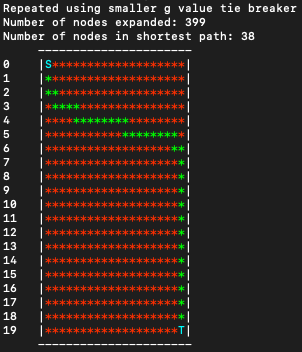
\includegraphics[width=.4\linewidth]{smaller-tie-breaker.png}
                        \caption{Tie breaker favoring smaller g-values}
                        \label{fig:sub1}
                    \end{subfigure}
                    \begin{subfigure}{.4\textwidth}
                        \centering
                        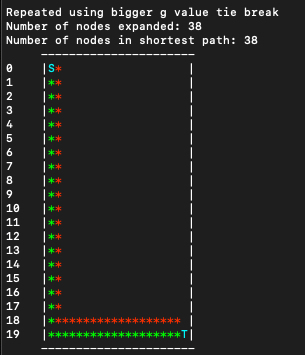
\includegraphics[width=.4\linewidth]{larger-tie-breaker.png}
                        \caption{Tie breaker favoring bigger g-values}
                        \label{fig:sub1}
                    \end{subfigure}
                    \caption{Tie breakers on g-values}
                    \label{tie-breaker}
                \end{figure}
                
            \end{enumerate}
        \item[3.] \textbf{Forward vs. Backward}
            \begin{enumerate}
                \item[] In the experiment, repeating forward A* expanded an average of 9702.88 nodes while repeating backwards A* expanded an average of 9351.14 nodes.  For this experiment, ties were broken in favor of cells with higher g values.  The fact that repeating forward A* ran slower than repeating backward A* must be a result of the mazes.  Since it is essentially the same algorithm with only the start and goals swapped, the only variant in the experiment is the makeup of the mazes, which were randomly generated.  Mazes with no solution may have been what caused the discrepancy as mazes with the the goal blocked off completely within a small corridor would take a very short time to run with repeating backward, while repeating forward would need to expand nearly every unblocked cell in the maze.
            \end{enumerate}
        \item[4.] \textbf{Heuristics in the Adaptive A* }
            \begin{enumerate}
                \item[] Suppose a worst case in which A needs to run A* after exploring each previously unexplored cell and A explores each unblocked cell before finding the target cell. This means A* is run by A a number of times equal to U. This means M can be defined by the equation M=M(i)*U. Since the statement  M(i)$\le$ U holds, the statement M= M(i)*U $\le$ U*U= $U^2$ is true, meaning M$\le$ $U^2$, or M=O($U^2$). 
            
            \item[ ] Manhattan distances are consistent in this problem because it gives the shortest path estimation, in which there's no obstacles between start and goal.
            Let g(s, s') is the cost reach state s' from s. In 2D gridworld, Manhattan distances h(s) fits in the triangle inequality: 
            
            \[h(s) \leq g(s, s') + h(s'). \]
            
            Therefore, Manhattan distances are always the best cost to reach from start to goal out of all actions and states we can go.

            For adaptive heuristics, by updating the new h values: 
            $h_{new}(s) = g(s_{goal}) - g(s)$ \par

            $h_{new}(s)$ still satisfies admissibility by not overestimate the path costs.

            \textbf{Proving $h_{new}(s)$ is consistent:} \par
            Has shortest cost to goal $g(s_{goal})$ is shortest comparing with any combination of g(s') and heuristics h(s'). Comparing s' with another state s, subtract cost to reach s from start by both sides. We obtain that $h_{new}(s)$ is consistent.
            
            \[g(s_{goal}) \leq g(s') + h(s') \] 
            \[g(s_{goal}) - g(s) \leq g(s') - g(s) + h(s') \] 
            \[h_{new}(s) \leq g(s,s') + h(s') \leq g(s,s') + h_{new}(s') \]         

            By the above inequation, it is guaranteed that $h_{new}(s)$ is consistent either comparing with an s' state also has been expanded (s' state had its h-new(s')) or comparing with an s' state that has never been expanded.
                
            \end{enumerate}
        \item[5.] \textbf{Heuristics in the Repeated A*}
            \begin{enumerate}
                \item[] In this experiment, repeating forward A* expanded an average of 9351.14 nodes while adaptive forward A* expanded an average of 8466.4 nodes.  Based on these results, adaptive forward A* is about 8 \% more efficient.  This makes sense based on the idea of adaptive A* making the expansion more focused since the heuristic is updated in favor of cells in the direction of the target while the heuristic in repeated A* never changes.  When the step cost begins to get very high relative to even the heuristic of cells that are not in the direction of the goal, A* will expand cells farther away because the step cost has grown higher than the heuristic of cells close to the start, whereas in adaptive A*, this is rarely the case since the heuristic is updated.
            \end{enumerate}
        \item[6.] \textbf{Statistical Significance}\begin{enumerate}
            \item[]Hypothesis Testing whether Adaptive A* is faster than Repeated Forward A*
            \item[$H_0$:]Adaptive A* is faster than Repeated Forward A* on average.
            \item[$H_1$:] Adaptive A* is not faster than Repeated Forward A* on average.
            \item[Test Proposal:] One statistical hypothesis test that could be performed to test the hypothesis that Adaptive A* is faster than Repeated Forward A* is the t-test. The t-test would be the best suited test for this data set because it is used to compare the means between two groups, such as the mean cell expansions between a group of paths found with Adaptive A* and a group of paths found with Repeated Forward A*. The t-test also requires the data be independent, approximately normally distributed, and possess a homogeneity of variance between each group. All of the paths in both groups were found independently of one another. Additionally, since the starting location and the ending location of each graph is selected randomly, the distance between these two points would also be random, meaning these distances, and thus the number of cells expanded to find an answer, would be approximately normally distributed. Finally, since both Adaptive A* and Repeated Forward A* are run on each map, each point in each group would have a similar data point in the other group, meaning the variance of the two points is approximately equal. Since the data is independent, approximately normally distributed, and has homogeneity of variance, a t-test would be appropriate for Statistical Hypothesis testing. Since for each data point in each group there exists a data point in the other group gathered from the same map with the same start and end points, a paired t-test would be appropriate to conduct. Additionally, since the purpose of the test is to discover if Adaptive A* is faster than Repeated Forward A*, a one-tailed t-test would be best. 
        \end{enumerate}
    \end{enumerate}


\end{document}
